% vim: set spell spelllang=en tw=100 et sw=4 sts=4 foldmethod=marker foldmarker={{{,}}} :

\documentclass{beamer}

\usepackage{tikz}
\usepackage{xcolor}
\usepackage{complexity}
\usepackage{hyperref}
\usepackage{microtype}
\usepackage{amsmath}                   % \operatorname
\usepackage{amsfonts}                  % \mathcal
\usepackage{amssymb}                   % \nexists
\usepackage{gnuplot-lua-tikz}          % graphs
\usepackage[vlined]{algorithm2e} % algorithms

\usetikzlibrary{shapes, arrows, shadows, calc, positioning, fit}
\usetikzlibrary{decorations.pathreplacing, decorations.pathmorphing, shapes.misc}
\usetikzlibrary{tikzmark}

\newcommand*\circled[1]{\tikz[baseline=(char.base)]{
            \node[shape=circle,draw,inner sep=0pt] (char) {#1};}}

\definecolor{uofguniversityblue}{rgb}{0, 0.219608, 0.396078}

\definecolor{uofgheather}{rgb}{0.356863, 0.32549, 0.490196}
\definecolor{uofgaquamarine}{rgb}{0.603922, 0.72549, 0.678431}
\definecolor{uofgslate}{rgb}{0.309804, 0.34902, 0.380392}
\definecolor{uofgrose}{rgb}{0.823529, 0.470588, 0.709804}
\definecolor{uofgmocha}{rgb}{0.709804, 0.564706, 0.47451}

\definecolor{uofglawn}{rgb}{0.517647, 0.741176, 0}
\definecolor{uofgcobalt}{rgb}{0, 0.615686, 0.92549}
\definecolor{uofgturquoise}{rgb}{0, 0.709804, 0.819608}
\definecolor{uofgsunshine}{rgb}{1.0, 0.862745, 0.211765}
\definecolor{uofgpumpkin}{rgb}{1.0, 0.72549, 0.282353}
\definecolor{uofgthistle}{rgb}{0.584314, 0.070588, 0.447059}
\definecolor{uofgpillarbox}{rgb}{0.701961, 0.047059, 0}
\definecolor{uofglavendar}{rgb}{0.356863, 0.301961, 0.580392}

% {{{ theme things
\useoutertheme[footline=authortitle]{miniframes}
\useinnertheme{rectangles}

\setbeamerfont{block title}{size={}}
\setbeamercolor*{structure}{fg=uofguniversityblue}
\setbeamercolor*{palette primary}{use=structure,fg=black,bg=white}
\setbeamercolor*{palette secondary}{use=structure,fg=black,bg=uofgcobalt}
\setbeamercolor*{palette tertiary}{use=structure,fg=white,bg=uofguniversityblue}
\setbeamercolor*{palette quaternary}{fg=white,bg=black}

\setbeamercolor*{titlelike}{parent=palette primary}

\beamertemplatenavigationsymbolsempty

\setbeamertemplate{title page}
{
    \begin{tikzpicture}[remember picture, overlay]
        \node [anchor=center, fill=white, fill opacity=0.8, text opacity=1, inner sep=0.2cm, shift={(0cm,0.3cm)}] at (current page.center) {
            \begin{minipage}{\paperwidth}
                \centering
                {\usebeamerfont{title}\inserttitle}
                \vskip0.2cm
                {\usebeamerfont{author}\insertauthor \quad \insertinstitute}
            \end{minipage}
        };
    \end{tikzpicture}

    \begin{tikzpicture}[remember picture, overlay]
        \node at (current page.north west) {\begin{tikzpicture}[remember picture, overlay]\fill
        [fill=uofguniversityblue, anchor=north west] (0, 0) rectangle (\paperwidth, -1.5cm);\end{tikzpicture}};
        \node [anchor=north west, shift={(0.2cm,-0.2cm)}] at (current page.north west) {\includegraphics*[keepaspectratio=true,scale=0.5]{UoG_keyline.pdf}};
    \end{tikzpicture}
}

\setbeamertemplate{section page}
{
    \begin{centering}
        \begin{beamercolorbox}[sep=12pt,center]{part title}
            \usebeamerfont{section title}\insertsection\par
        \end{beamercolorbox}
    \end{centering}
}

\newcommand{\frameofframes}{/}
\newcommand{\setframeofframes}[1]{\renewcommand{\frameofframes}{#1}}

\makeatletter
\setbeamertemplate{footline}
{%
    \begin{beamercolorbox}[colsep=1.5pt]{upper separation line foot}
    \end{beamercolorbox}
    \begin{beamercolorbox}[ht=2.5ex,dp=1.125ex,%
        leftskip=.3cm,rightskip=.3cm plus1fil]{author in head/foot}%
        \leavevmode{\usebeamerfont{author in head/foot}\insertshortauthor}%
        \hfill%
        {\usebeamerfont{institute in head/foot}\usebeamercolor[fg]{institute in head/foot}\insertshortinstitute}%
    \end{beamercolorbox}%
    \begin{beamercolorbox}[ht=2.5ex,dp=1.125ex,%
        leftskip=.3cm,rightskip=.3cm plus1fil]{title in head/foot}%
        {\usebeamerfont{title in head/foot}\insertshorttitle}%
        \hfill%
        {\usebeamerfont{frame number}\usebeamercolor[fg]{frame number}\insertframenumber~\frameofframes~\inserttotalframenumber}
    \end{beamercolorbox}%
    \begin{beamercolorbox}[colsep=1.5pt]{lower separation line foot}
    \end{beamercolorbox}
}

% }}}

\title{A Parallel, Backjumping Subgraph Isomorphism Algorithm using Supplemental Graphs}
\author{Ciaran McCreesh and Patrick Prosser}

\begin{document}

{
    \usebackgroundtemplate{
        \tikz[overlay, remember picture]
        \node[at=(current page.south), anchor=south, inner sep=0pt]{\includegraphics*[keepaspectratio=true, width=\paperwidth]{background.jpg}};
    }
    \begin{frame}[plain,noframenumbering]
        \titlepage
    \end{frame}
}

\section{Subgraph Isomorphism}

\begin{frame}{The Subgraph Isomorphism Problem}

    \centering
    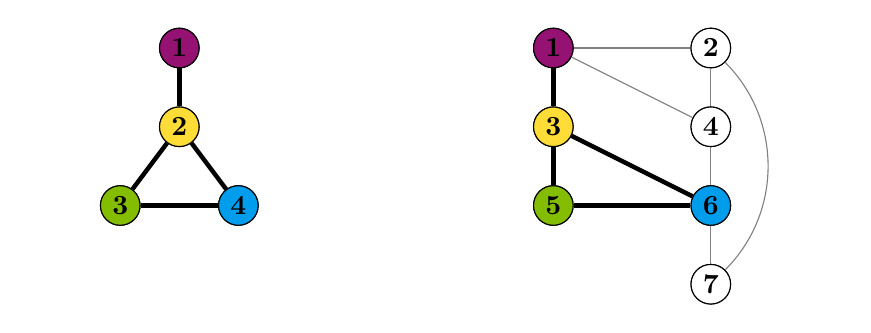
\begin{tikzpicture}%{{{
        \node at (-1, 0) { ~ };
        \node at (9, 0) { ~ };

        \node <1> [draw, circle, fill=white, inner sep=2pt, font=\bfseries] (Na) at (0.75,  0) {1};
        \node <1> [draw, circle, fill=white, inner sep=2pt, font=\bfseries] (Nb) at (0.75, -1) {2};
        \node <1> [draw, circle, fill=white, inner sep=2pt, font=\bfseries] (Nc) at (0, -2) {3};
        \node <1> [draw, circle, fill=white, inner sep=2pt, font=\bfseries] (Nd) at (1.5, -2) {4};

        \node <2> [draw, circle, fill=uofgthistle, inner sep=2pt, font=\bfseries] (Na) at (0.75,  0) {1};
        \node <2> [draw, circle, fill=uofgsunshine, inner sep=2pt, font=\bfseries] (Nb) at (0.75, -1) {2};
        \node <2> [draw, circle, fill=uofglawn, inner sep=2pt, font=\bfseries] (Nc) at (0, -2) {3};
        \node <2> [draw, circle, fill=uofgcobalt, inner sep=2pt, font=\bfseries] (Nd) at (1.5, -2) {4};

        \tikzstyle{edge} = [ultra thick];
        \tikzstyle{ledge} = [color = black!50!white];

        \draw <1> [ledge] (Na) -- (Nb);
        \draw <1> [ledge] (Nb) -- (Nc);
        \draw <1> [ledge] (Nc) -- (Nd);
        \draw <1> [ledge] (Nb) -- (Nd);

        \draw <2> [edge] (Na) -- (Nb);
        \draw <2> [edge] (Nb) -- (Nc);
        \draw <2> [edge] (Nc) -- (Nd);
        \draw <2> [edge] (Nb) -- (Nd);

        \node <1> [draw, circle, fill=white, inner sep=2pt, font=\bfseries] (N1) at (5.5,  0) {1};
        \node <1> [draw, circle, fill=white, inner sep=2pt, font=\bfseries] (N2) at (7.5,  0) {2};
        \node <1> [draw, circle, fill=white, inner sep=2pt, font=\bfseries] (N3) at (5.5, -1) {3};
        \node <1> [draw, circle, fill=white, inner sep=2pt, font=\bfseries] (N4) at (7.5, -1) {4};
        \node <1> [draw, circle, fill=white, inner sep=2pt, font=\bfseries] (N5) at (5.5, -2) {5};
        \node <1> [draw, circle, fill=white, inner sep=2pt, font=\bfseries] (N6) at (7.5, -2) {6};
        \node <1> [draw, circle, fill=white, inner sep=2pt, font=\bfseries] (N7) at (7.5, -3) {7};

        \node <2> [draw, circle, fill=uofgthistle, inner sep=2pt, font=\bfseries] (N1) at (5.5,  0) {1};
        \node <2> [draw, circle, fill=white, inner sep=2pt, font=\bfseries] (N2) at (7.5,  0) {2};
        \node <2> [draw, circle, fill=uofgsunshine, inner sep=2pt, font=\bfseries] (N3) at (5.5, -1) {3};
        \node <2> [draw, circle, fill=white, inner sep=2pt, font=\bfseries] (N4) at (7.5, -1) {4};
        \node <2> [draw, circle, fill=uofglawn, inner sep=2pt, font=\bfseries] (N5) at (5.5, -2) {5};
        \node <2> [draw, circle, fill=uofgcobalt, inner sep=2pt, font=\bfseries] (N6) at (7.5, -2) {6};
        \node <2> [draw, circle, fill=white, inner sep=2pt, font=\bfseries] (N7) at (7.5, -3) {7};

        \draw [ledge] (N1) -- (N2);
        \draw [ledge] (N1) -- (N4);
        \draw [ledge] (N2) -- (N4);
        \draw [ledge] (N4) -- (N6);
        \draw [ledge] (N2) to [in=45, out=315] (N7);
        \draw [ledge] (N6) -- (N7);

        \draw <1> [ledge] (N1) -- (N3);
        \draw <1> [ledge] (N3) -- (N5);
        \draw <1> [ledge] (N3) -- (N6);
        \draw <1> [ledge] (N5) -- (N6);
        \draw <2> [edge] (N1) -- (N3);
        \draw <2> [edge] (N3) -- (N5);
        \draw <2> [edge] (N3) -- (N6);
        \draw <2> [edge] (N5) -- (N6);

    \end{tikzpicture}%}}}
    \\~

\end{frame}

\begin{frame}{Applications}
    \begin{itemize}
        \item Bioinformatics and chemistry.
        \item Computer vision and pattern recognition.
        \item Fraud detection and law enforcement.
        \item Model checking.
        \item Social network analysis.
        \item Diseased cows.
    \end{itemize}
\end{frame}

\begin{frame}{The Basic CP Model}
    \begin{itemize}
        \item One variable for each vertex in the pattern graph, with the domains being the vertices
            of the target graph.
        \item If two vertices are adjacent in the pattern, they must be mapped to adjacent vertices
            in the target.
            \begin{itemize}
                \item In the \emph{induced} variant, non-adjacent vertices must be mapped to
                    non-adjacent vertices. We only discuss the non-induced variant in this talk.
            \end{itemize}
        \item All pattern vertices must be given different values.
        \item Often enhanced: for example, we can filter based upon degree.
    \end{itemize}
\end{frame}

\begin{frame}{Another Perspective}
    \begin{itemize}
        \item The variables describe an injective mapping from the pattern to the target, which
            preserves adjacency.
    \end{itemize}

    \[
        P \rightarrowtail T
    \]
\end{frame}

\begin{frame}{Selected Previous Work}
    \begin{itemize}
        \item VF2: backtracking search, interesting heuristics. \\[0.1cm]
            {\scriptsize A (Sub)Graph Isomorphism Algorithm for Matching Large Graphs. Luigi P.
            Cordella and Pasquale Foggia and Carlo Sansone and Mario Vento. {IEEE} Trans.
        Pattern Anal. Mach. Intell., 2004.}

        \item LAD: locally all-different, and neighbourhood degree sequences. \\[0.1cm]
            {\scriptsize AllDifferent-based filtering for subgraph isomorphism. Christine Solnon.
            Artif. Intell., 2010.}
        \item SND: distance-based filtering. \\[0.1cm]
            {\scriptsize Scoring-Based Neighborhood Dominance for the Subgraph Isomorphism Problem.
            Gilles Audemard and Christophe Lecoutre and Mouny Samy Modeliar and Gilles
        Goncalves and Daniel Porumbel. CP 2014.}
    \end{itemize}
\end{frame}

\begin{frame}{Being Clever is Expensive}
    \begin{itemize}
        \item We want to work with up to 1,000 pattern vertices, and 10,000 target vertices.

        \item When LAD and SND fail, they often manage less than one recursive call per second,
            particularly with larger target graphs.
    \end{itemize}
\end{frame}

\section{Our Algorithm}
\frame{\sectionpage}

\begin{frame}{Our Approach}
    \begin{itemize}
        \item Cheaper inference: $10^4$ to $10^6$ recursive calls per second.
        \item Expensive preprocessing once at the top of search, rather than computing distances and
            degree sequences during search.
        \item FC-CBJ instead of MAC:
            \begin{itemize}
                \item A counting-based bit-parallel all-different propagator, which does more
                    than pairwise-$\ne$ AC but less than GAC.
                \item CBJ without explicit conflict sets, and without modifying propagators.
            \end{itemize}
        \item Thread-parallel search:
            \begin{itemize}
                \item Safe, deterministic search via nested parallel folds.
                \item Explicit early work-stealing, to fake discrepancy search.
            \end{itemize}
    \end{itemize}
\end{frame}

\begin{frame}{Supplemental Graphs}
    \only<1> {
        \begin{itemize}
            \item Adjacent vertices must be mapped to adjacent vertices.
            \item Used by SND:
                \begin{itemize}
                    \item Vertices that are distance 2 apart must be mapped to vertices that are within
                        distance 2.
                    \item Vertices that are distance $k$ apart must be mapped to vertices that are within
                        distance $k$.
                \end{itemize}
        \end{itemize}
    }

    \only<2> {
        \begin{itemize}
            \item A subgraph isomorphism

        \[
            f : P \rightarrowtail T
        \]

        is also a subgraph isomorphism

        \[
            f^2 : P^2 \rightarrowtail T^2
        \]

        and a subgraph isomorphism

        \[
            f^3 : P^3 \rightarrowtail T^3
        \]
        \end{itemize}
    }

    \only<3> {
        \begin{itemize}
            \item We can do something stronger: rather than looking at distances, we can look at
                (simple) paths, and we can count how many there are.

            \item This is \NP-hard in general, but only lengths 2 and 3 and counts of 2 and 3 are
                useful in practice.

            \item We construct these graph pairs once, at the top of search, and use them for
                degree-based filtering and during search.

            \item We get lots of implied constraints.
        \end{itemize}
    }
\end{frame}

\begin{frame}{Counting-Based All-Different}
    \begin{itemize}
        \item \emph{If it looks like I'll have lots of time: explain and animate this}
    \end{itemize}
\end{frame}

\begin{frame}{Backjumping}
    \begin{itemize}
        \item Rather than backtracking on failure, we can sometimes show it's safe to jump back
            several levels immediately.
        \item This can be done with without explicit conflict sets, and without modifying
            propagators.
        \item See the paper for details.
    \end{itemize}
\end{frame}

\begin{frame}{Sequential Experiments}
    \begin{itemize}
        \item 2,487 pairs of instances, selected by other people:
            \begin{itemize}
                \item Real-world graphs.
                \item 2D images and 3D meshes from computer vision applications.
                \item Random (simple, scale-free, 4D mesh, bounded degree).
            \end{itemize}

        \item A mix of satisfiable and unsatisfiable instances, although there is a bias towards
            satisfiable instances\ldots

        \item Up to 900 vertices and 12,410 edges in the pattern, and 5,944 vertices and 34,210
            edges in a target.

        \item Dual Intel Xeon E5-2640 v2 (Q3'13), 64GBytes RAM.

        \item Our code is C++, LAD and VFLib are C, SND is Java.
    \end{itemize}
\end{frame}

\begin{frame}{Cumulative Instances Solved}
    \only<1>{
        \input{gen-graph-cumulative-0}
    }
    \only<2>{
        \input{gen-graph-cumulative-1}
    }
    \only<3>{
        \input{gen-graph-cumulative-2}
    }
    \only<4>{
        \input{gen-graph-cumulative-3}
    }
    \only<5>{
        \input{gen-graph-cumulative-4}
    }
    \only<6>{
        \input{gen-graph-cumulative-5}
    }
\end{frame}

\begin{frame}{Versus Virtual Best Other Solver}
    \only<1>{
        \input{gen-graph-best-other-0}
    }
    \only<2>{
        \input{gen-graph-best-other-1}
    }
\end{frame}

\begin{frame}{Backjumping?}
    \only<1>{
        \input{gen-graph-backjumping-0}
    }
    \only<2>{
        \input{gen-graph-backjumping-1}
    }
\end{frame}

\begin{frame}{Counting All-Different?}
    \only<1>{
        \input{gen-graph-fad-0}
    }
    \only<2>{
        \input{gen-graph-fad-1}
    }
    \only<3>{
        \input{gen-graph-fad-2}
    }
\end{frame}

\section{Thread Parallelism}
\frame{\sectionpage}

\begin{frame}{Parallel Preprocessing}
    \begin{itemize}
        \item Entirely (mostly\ldots) routine and not very interesting, but good at offsetting the
            cost of supplemental graph construction.
    \end{itemize}
\end{frame}

\begin{frame}{Parallel Tree-Search}
    \begin{itemize}
        \item Explicit early-first work stealing, to offset incorrect decisions early in search.
            \begin{itemize}
                \item There are EHPs, and this gets rid of them more cheaply than discrepancy
                    searches.
            \end{itemize}
        \item Backjumping is a nested parallel fold with left-zero elements.
        \item Speculative, so we should not expect linear speedups (even on unsat instances).
    \end{itemize}
\end{frame}

\begin{frame}{Sidenote on Safety, Parallelism, and Benchmarking}
    \begin{itemize}
        \item Parallel search will never be substantially worse than sequential search.
        \item Adding more cores will never make things substantially worse (excluding
            hardware weirdness).
        \item Running it twice will give more or less the same runtimes.
        \item All comparisons are against a dedicated sequential implementation of a strong
            algorithm, not a threaded implementation run with one thread.
    \end{itemize}
\end{frame}

\begin{frame}{Parallel Experiments}
    \begin{itemize}
        \item 2 CPUs, 8 cores per CPU, hyper-threaded, so 32 software threads.
        \item We do \emph{not} have 32 times the computation power, and only about twice the memory
            bandwidth\ldots
    \end{itemize}
\end{frame}

\begin{frame}{Speedups}
    \only<1>{
        \input{gen-graph-speedup-0}
    }
    \only<2>{
        \input{gen-graph-speedup-1}
    }
\end{frame}

\begin{frame}{Is Comparing Sequential and Parallel Solvers Fair?}
    \begin{itemize}
        \item Personal view: single-threaded for understanding ``inside search'' behaviour,
            but ``horse race'' benchmarks should be a free-for-all.

        \item You're paying for multi-core even if you aren't using it.

        \item Java uses multiple cores even for sequential code, so the sequential benchmarks were
            unfair.

        \item You are welcome to disagree, and ignore the following two slides.
    \end{itemize}
\end{frame}

\begin{frame}{Cumulative Instances Solved}
    \only<1>{
        \input{gen-graph-cumulative-4}
    }
    \only<2>{
        \input{gen-graph-cumulative-6}
    }
    \only<3>{
        \input{gen-graph-cumulative-7}
    }
\end{frame}

\begin{frame}{Versus Virtual Best Other Solver}
    \only<1>{
        \input{gen-graph-best-other-1}
    }
    \only<2>{
        \input{gen-graph-best-other-2}
    }
\end{frame}

\section{Future Work}
\frame{\sectionpage}

\begin{frame}{Conspicuously Absent From This Talk}
    \begin{itemize}
        \item Labels? Directed edges? Induced? Wildcards?

        \item Why that choice of supplemental graphs, using only paths of lengths 2 and 3? It seems
            rather arbitrary. Can we do better with domain knowledge, or with portfolios?

        \item Why does that counting all-different propagator do so well in practice? Is it only
            subgraph isomorphism where it helps?
    \end{itemize}
\end{frame}

\begin{frame}
    \begin{center}
        Reproduce, replicate, or recompute this paper: \\
        \url{http://dcs.gla.ac.uk/~ciaran} \\
        \vspace{1em}
        Tell me whether it worked: \\
        \href{mailto:c.mccreesh.1@research.gla.ac.uk}{\nolinkurl{c.mccreesh.1@research.gla.ac.uk}} \\
        \vspace{1em}
        Donate your subgraph isomorphism problem instances: \\
        \url{http://liris.cnrs.fr/csolnon/SIP.html}
\end{center}
\begin{tikzpicture}[remember picture, overlay]
    \node at (current page.north west) {\begin{tikzpicture}[remember picture, overlay]\fill
    [fill=uofguniversityblue, anchor=north west] (0, 0) rectangle (\paperwidth, -1.5cm);\end{tikzpicture}};
    \node [anchor=north west, shift={(0.2cm,-0.2cm)}] at (current page.north west) {\includegraphics*[keepaspectratio=true,scale=0.5]{UoG_keyline.pdf}};
\end{tikzpicture}
\end{frame}

\end{document}

